\chapter{La cryptographie à travers l'histoire}
Avant de commencer à décrire la cryptographie en soi, voyons un peu
son histoire, son apparition, et son évolution au fil du temps ; les
aspects techniques brièvement présentés dans ce chapitre seront
expliqué au cours des chapitres suivants.

\section{L'apparition de la cryptographie}
La cryptographie serait apparue pour la première fois il y a 4000 ans,
au bord du Nil, où un scribe aurait tracé d'une façon spéciale des
hiéroglyphes sur la tombe de son maître, bien que ce n'était pas
vraiment dans le but de rendre le texte illisible, mais de le rendre
plus solennel.

La seconde trace de cryptographie date du \bc{XVI}, c'est une tablette
d'argile sur laquelle un potier aurait écrit sa recette en enlevant
les consonnes et en changeant l'orthographe de certains mots. \\

À cette époque là, les seuls moyens utilisés pour cacher les messages
ressemblaient plus à de la stéganographie qu'à de la cryptographie,
les messages ne sont pas rendus illisibles, mais sont cachés. Par
exemple, aux alentours de -600, Nabuchodonosor rasait le crâne d'un
esclave, écrivait un message dessus, et une fois que les cheveux
avaient repoussé, l'esclave allait chez le destinataire du message,
qui lui rasait les cheveux pour le lire. Un autre exemple est celui
d'Harpage, qui était chargé de tuer Cyrus, le petit fils du roi de
Mèdes, mais qui ne le fit pas. Par la suite, quand Cyrus a grandi,
pour communiquer avec lui, Harpage cachait les lettres dans le ventre
de lièvres, qu'il recousait ensuite. De cette façon, le message passe
inaperçu. \\

Les premières « vraies » techniques de cryptographie apparaissent
quant à elles à partir du \bc{VI}, avec une méthode de substitution,
nommée \emph{atbash}, qui consiste à remplacer les lettres par la
lettre « opposée », c'est-à-dire que A sera remplacé par Z, B par Y,
et ainsi de suite.
\begin{figure}[h]
%\begin{wrapfigure}{l}{0.5\textwidth}
  \centering
%    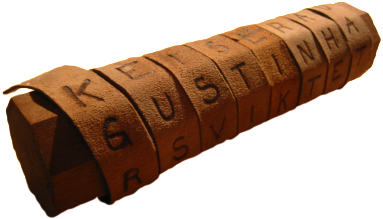
\includegraphics[scale=1]{images/Scytale.png}
%    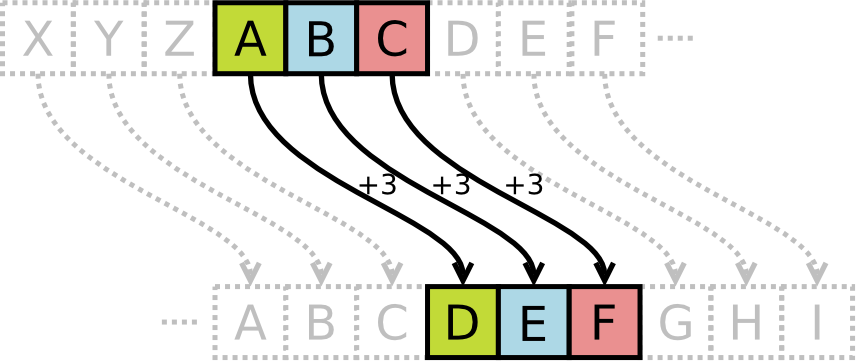
\includegraphics[scale=0.4]{images/ChiffreCesar.png}
    \subfloat[La scytale des spartiates]{
      \label{fig:Scytale}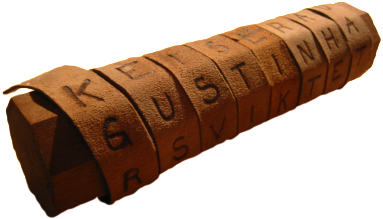
\includegraphics[width=0.4\textwidth]{images/Scytale.png}}
    \hspace{1.5cm}
    \subfloat[Le fonctionnement du chiffre de César]{
      \label{fig:Cesar}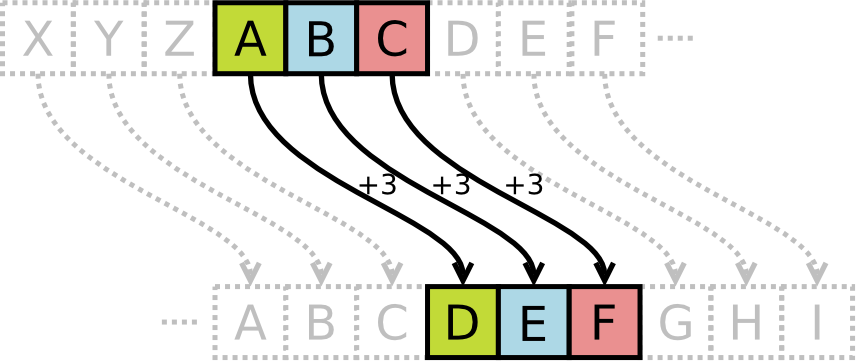
\includegraphics[width=0.4\textwidth]{images/ChiffreCesar.png}}
%    \vspace{-5pt}
    \caption{Deux anciennes techniques de chiffrement}
    \vspace{-15pt}
%  \label{fig:ScytaleChiffreCesar}
\end{figure}
%\end{wrapfigure}
% \begin{figure}[h]
%   \begin{center}
%     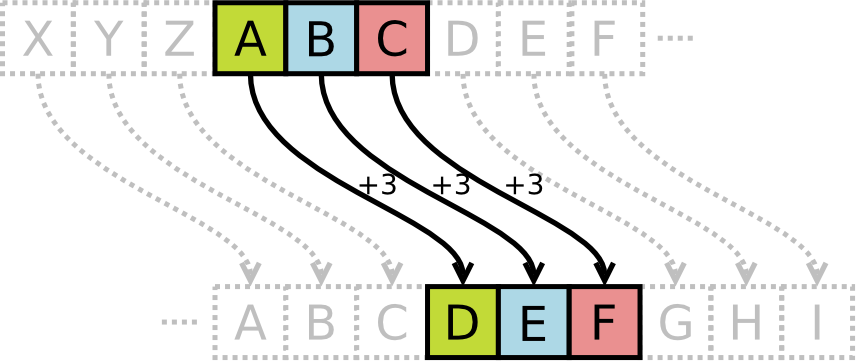
\includegraphics[scale=0.4]{images/ChiffreCesar.png}
%   \end{center}
%   \caption{Le chiffre de César}
%   \label{fig:ChiffreCesar}
% \end{figure}


  
Ensuite, au \bc{V}, les spartiates utilisaient pour communiquer le
bâton de Plutarque, plus connu sous le nom de \emph{scytale}. Cette
technique consistait à enrouler un long et étroit morceau de parchemin
autour d'un bâton, on écrivait ensuite le message sur le parchemin, et
on envoyait ce parchemin déroulé au destinataire, qui possédait un
bâton de même diamètre pour déchiffrer le message.

Le premier réel système cryptographique par substitution est inventé
par un historien grec, Polybe aux alentours de 150 avant J.-C. (nous
verrons ce système en détail dans le chapitre \ref{syst:CarrePolybe} (page
\pageref{syst:CarrePolybe}). \\

\label{syst:ChiffreCesar}
Pendant le \bc{I}, les armées de César utilisaient une méthode de
chiffrement par substitution simple, qui consistait à décaler les
lettres de l'alphabet d'un certain rang dans l'alphabet (de 3 rangs la
plupart du temps, ainsi A devient D, B devient E, \dots). Cette simple
méthode est une des méthodes de chiffrement les plus connues et à été
utilisée de nombreuses fois par la suite dans des formes dérivées (chiffre de
Vigenère\footref{syst:ChiffreVigenere}, rot13\footref{syst:rot13}), ou même
de la même façon (pendant la guerre de sécession par exemple).

Au Moyen-âge, comme la plupart des sciences, la cryptologie n'évolue
presque pas (une personne pratiquant la cryptologie peut être
considérée comme faisant de la magie noire), à part quelques exceptions
au Moyen-Orient et en Asie (dans le Kama-sutra, il est dit que les
femmes doivent apprendre le \emph{mlecchita-vikalpa} (l'art de
l'écriture secrète) pour cacher leurs liaisons.). Il faut donc
attendre le XV\ieme~siècle pour que la cryptographie commence
réellement à évoluer. \\

\section{L'évolution de la cryptographie}
Au début du XV\ieme~siècle donc, un égyptien écrit une encyclopédie
en 24 volumes comprenant une partie sur la cryptologie qui décrit des
chiffres de substitution et de transposition. Le premier chiffre de
substitution polyalphabétique\footref{SubstitutionPolyalphabetique}
est inventé par Leone Battista Alberti en 1467, un humaniste italien
de la renaissance, aussi connu pour ses travaux en architecture,
surnommé \emph{Le père de la cryptographie occidentale} par
l'historien David Kahn \cite{Codebreakers}. Cette technique est appelée
le \emph{cadran chiffrant}\label{syst:CadranChiffrant}, qui consiste
en deux disques attachés ensemble de façon à pouvoir coulisser,
contenant chacun les lettres de l'alphabet dans 24 cases (le premier
en contient 20, H, K et Y n'étant pas « indispensables », J, U et W
n'étant pas dans l'alphabet latin, les 4 autres cases sont occupées
par des chiffres. L'autre disque contient les 23 lettres latines dans
un ordre aléatoire et le signe \texttt{\&}). Le plus petit disque peut tourner,
les lettres claires et chiffrées se trouvent alors face à face, et il
suffit de recopier la lettre du petit disque pour chiffrer la lettre
du grand disque. Après avoir chiffré quelques lettres, on décale le
disque et on continue ainsi de suite, en indiquant sur le message
chiffré le changement. Dans son ouvrage, il parle aussi de
cryptanalyse, et il introduit le concept d'analyse des
fréquences. \\

\begin{figure}[h]
  \begin{center}
    \subfloat[Le cadran chiffrant d'Alberti dans sa forme originelle]{
      \label{fig:CadranChiffrant}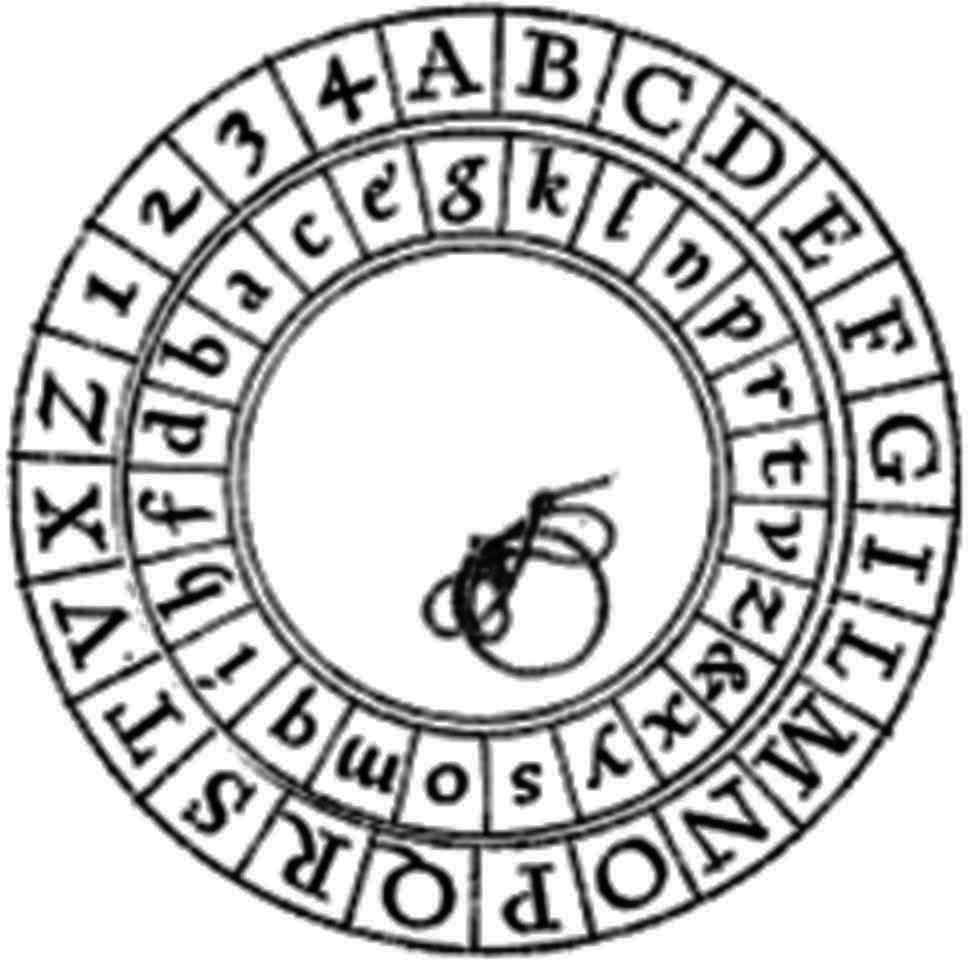
\includegraphics[width=0.4\textwidth]{images/AlbertiCipherDisk.jpg}}
    \hspace{1.5cm}
    \subfloat[Le cadran chiffrant réutilisé par les confédérés pendant
    la guerre de sécession]{
      \label{fig:CadranConfederes}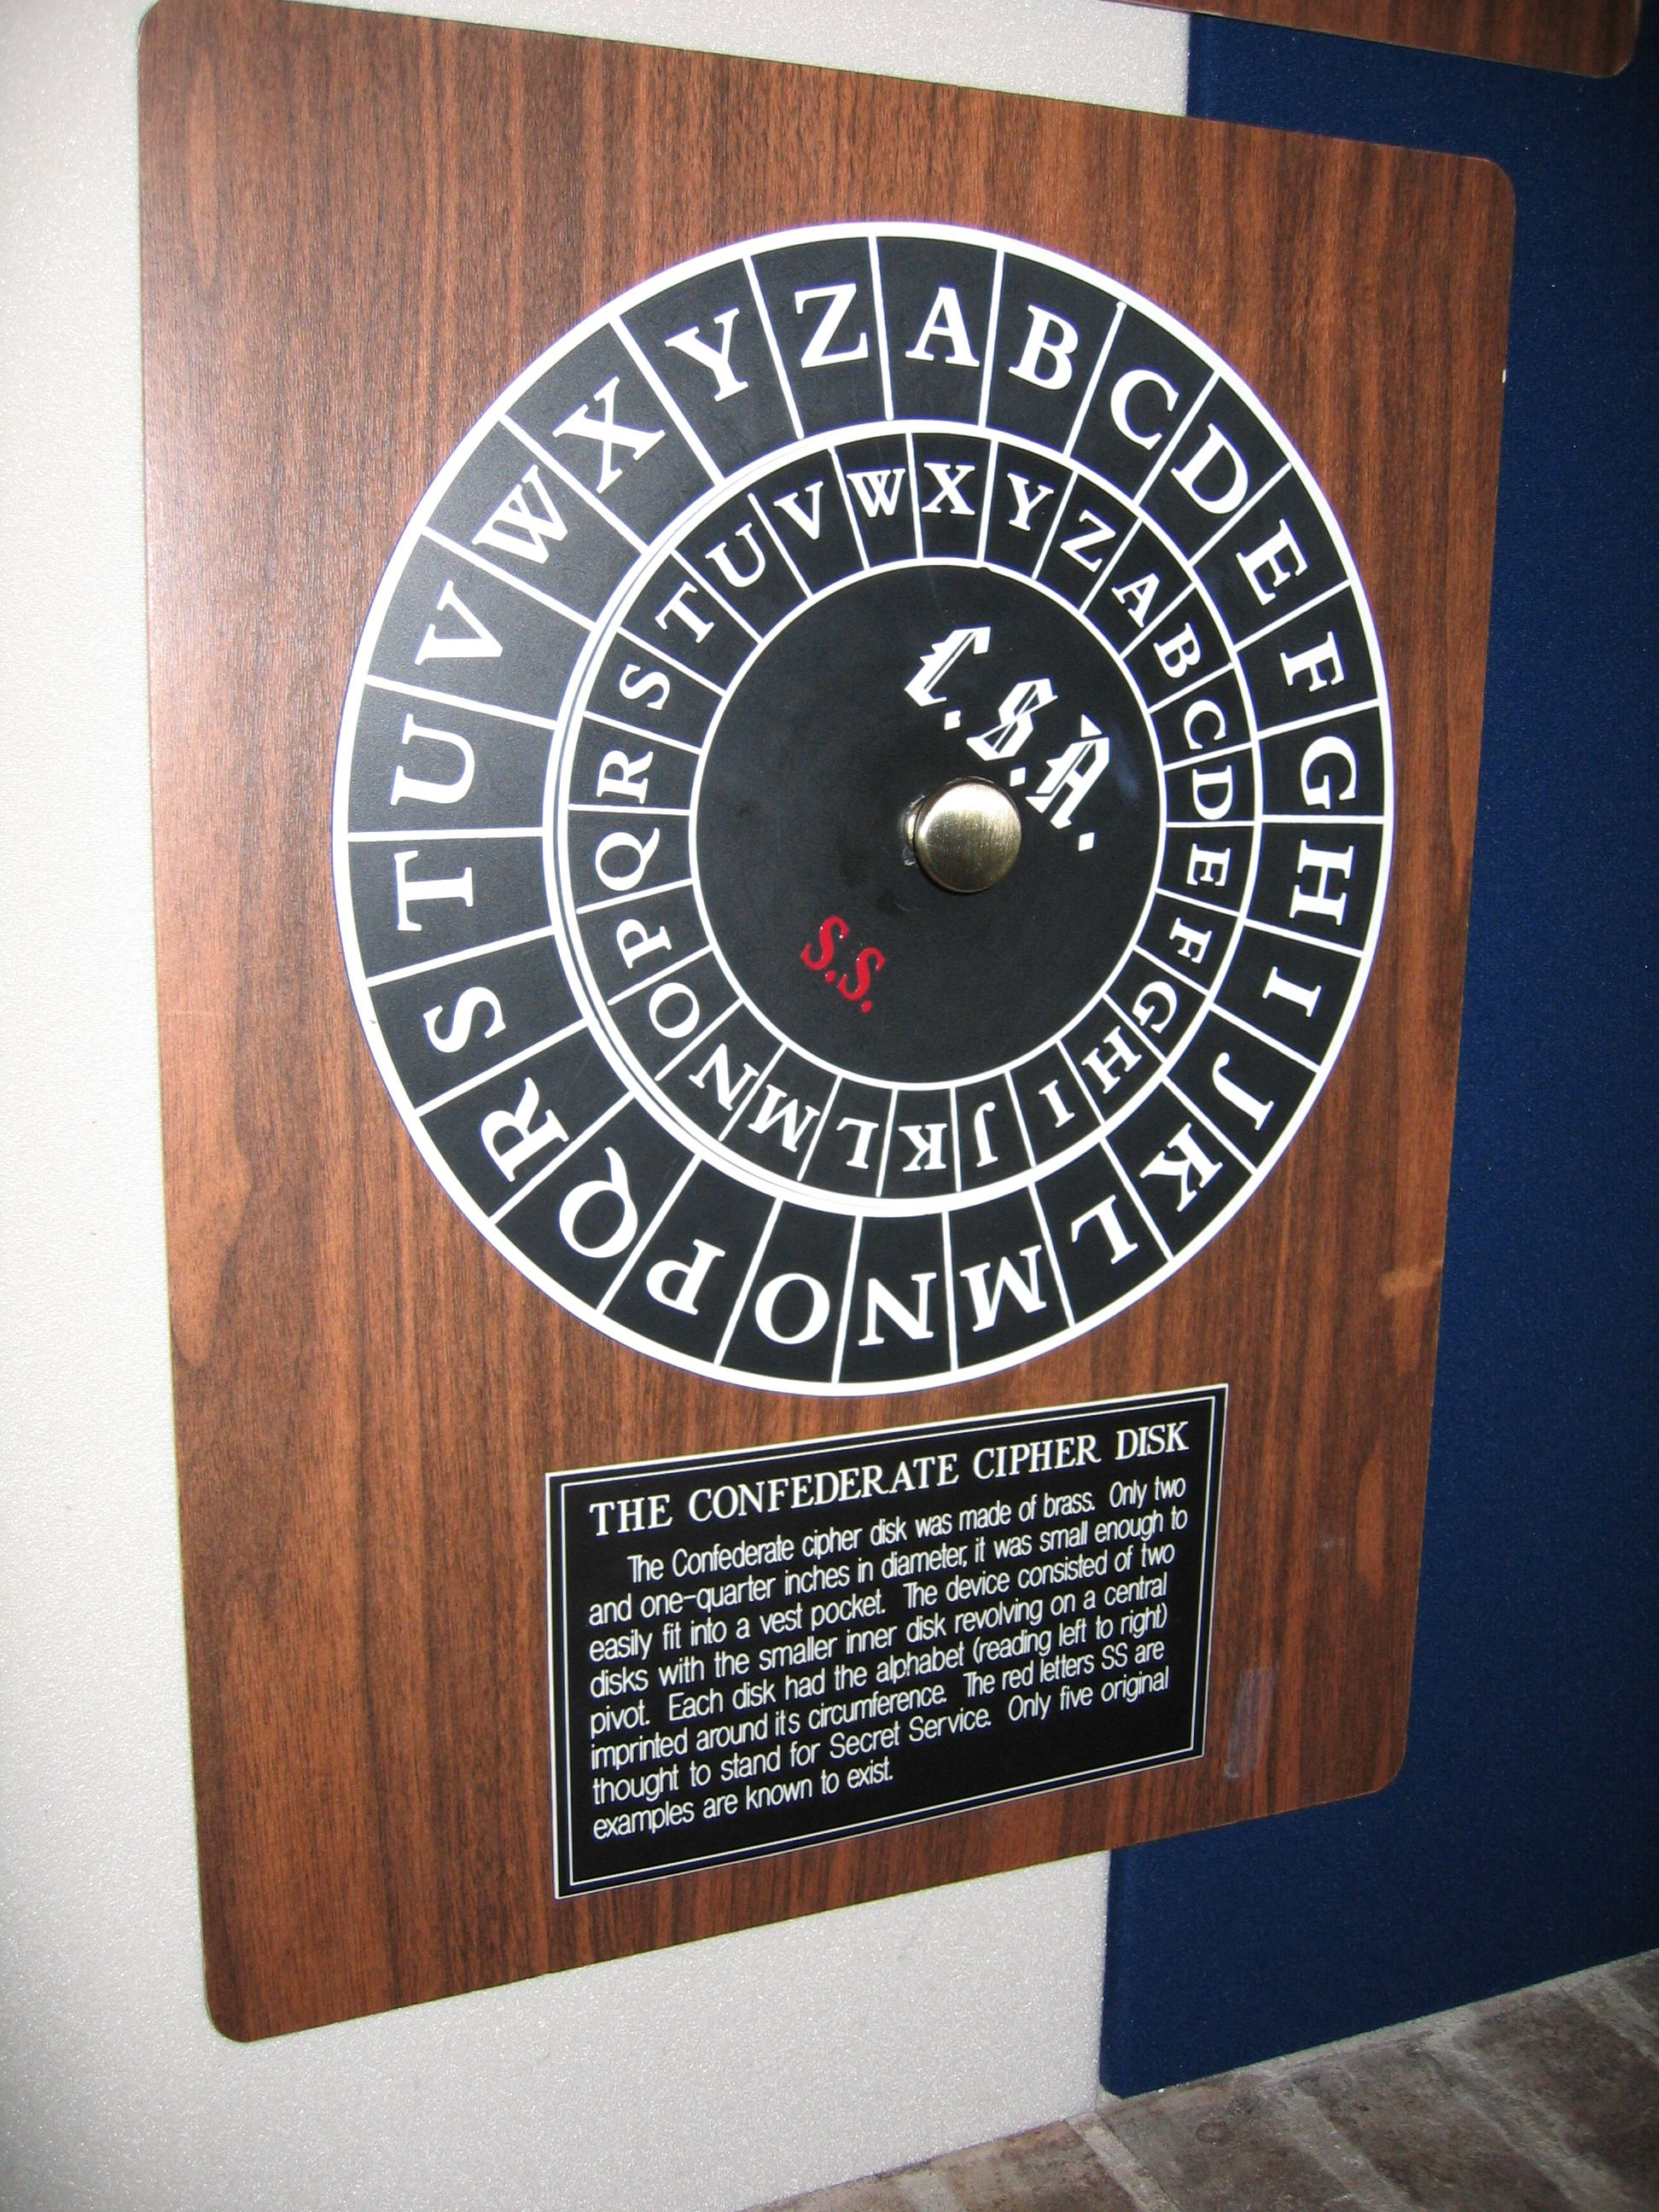
\includegraphics[width=0.4\textwidth]{images/ConfederateCipherDisk.jpg}}

  \end{center}
  \vspace{-10pt}
  \caption{Cadrans chiffrants}
  \vspace{-15pt}
\end{figure}

En 1518, Jean Trithème publie \emph{Polygraphi\ae} , le premier livre imprimé
sur la cryptologie, où il invente un chiffre stéganographique, et ce
qui deviendra par la suite le chiffre de
Vigenère. \\

Au milieu du XVI\ieme~siècle, Jérôme Cardan invente le premier
\emph{procédé autoclave} (qui utilise le message clair comme clef),
mais ce système comporte des lacunes. Il invente aussi la \emph{grille
  de Cardan}, un système stéganographique qui cache un message dans
une grille de lettres. Pour lire le message, il faut utiliser un cache
troué d'une certaine façon, les lettres apparaissent alors dans les
trous, et on peut lire le message. \\

%\begin{figure}[h]
\begin{wrapfigure}{L}{0.5\textwidth}
  \begin{center}
    \includegraphics[scale=0.2]{images/GrilleCardan.png}
  \end{center}
  \caption{Un exemple de grille de Cardan}
  \label{fig:GrilleCardan}
  \vspace{-10pt}
%\end{figure}
\end{wrapfigure}

% Premières techniques de cryptographie
% Plus vieux document chiffré : un potier qui écrit sa recettes en
% enlevant des consonnes et en changeant l'orthographe des mots.
% En chine : stégano (papirus enroulé en boule recouvert de cire, avalé)
% première trace : vers 2000 av J.-C.
% Scytale -500 av J.-C. : == bâton de Plutarque.
% Spartiates, bâton rond, qu'on entoure d'un long et étroit morceau de
% parchemin. Une fois mis autour, on écrit le message dessus, puis on
% l'envoie au destinataire, qui possède une scytale de même diamètre,
% et qui déchiffre donc facilement le message. Fa
% Nabuchodonosor : -600 av J.-C. : 
% On rase le crâne d'un esclave, et une fois les cheveux repoussés, on
% l'envoie au destinataire, qui rase à nouveau les cheveux.
% Harpage qui envoie un message à Cyrus, il ouvre le ventre d'un
% lièvre pour y cacher une lettre, et l'envoya à Cyrus.
% Hebreux : Vieme av JC, atbash, chaque lettre est inversée A->Z,
% B->Y, ...

% ~-200 : premiers "vrais" systèmes cryptographiques : 
% caré de polybe, historiengrec : ~-150
% 1er siècle avant J.-C. : 
% code de césar utilisé dans l'armée romaine, réutilisé par la suite
% durant la guerre de sécession et l'armée russe en 1915 (rot13)

% Moyen age : quasi rien car sorcellerie, tout ça.

% Quasi rien jusqu'au XVieme 
%XV : encyclopédie de 14 volume écrite par un égyptien Abd Allah
%al-Qalashandi qui inclut une section sur la cryptologie. Elle y
%décrit des chiffres de substitution et de transposition.
% Leon Battista Alberti, humaniste italien de la renaissance,
% architecte, écrivain, philosophe et peintre. IMAGE
% écrit un essai parlant de cryptanalyse, avec
% l'analyse de fréquences des lettres en latin et italien. Invente
% aussi le cadran chiffrant, première méthode de chiffrement
% polyalphabétique.
% Cadran chiffrant : 2 disques contenant les lettres de l'alphabet, 
%dont un qui tourne (20 lettres chez Alberti, et le cadran faisait 24
%cases, JUW pas dans l'alphabet, et on omet H et K et Y (« qui ne sont pas
%indispensables », le deuxième cadran contient les 23 lettres latines
%+ le &) Après avoir chiffré 3 ou 4 lettres, on décale le disque, et
%on l'indique en notant de le message la lettre au dessus du k(lettre
%sur le petit).
% Notion de surchiffrement aussi. (à relire)

% 1518 : Jean trithème écrit Polygraphiae, premier livre imprimé sur
% la cryptologie, où il invente un chiffre stéganographique et ce qui
% deviendra par la suite le chiffre de Vigenère. voir la bonne partie

% Pendant certaines guerres en europe, les espagnols communiquaient
% via un chiffre, qu'ils changaient de temps en temps afin de troubler
% les gens qui pourraient essayer de le déchiffrer. Certaines lettres
% furent interceptés, et Henri IV chargea un géomètre, Viete, de
% trouver la clé de ces lettres. Il y réussit brillement, en
% comprenant le chiffre dans toutes ses formes possibles. La Cour
% d'Espagne, accusa le gouvernement français d'avoir recouru à des
% serciers, et voulait que Viete soit jugé comme un négromant en
% portant des plaintes à Rome. Il n'en fut rien mais à cette époque
% encore, c'était très dangereux d'être considéré comme un sorcier.

% Milieu du 16ème, Jérôme cardan invente le premier procédé autoclave,
% et une méthode stéganographique connue sous le nom de grille de
% cardan, où il cache le message dans une "grille de lettres", on
% retrouvera le message facilement 


En 1553, Giovan Batista Belaso utilise le terme \emph{clé littérale}
ou \emph{mot de passe} pour des clés de petite taille faciles à
mémoriser. %TODO: plus d'infos
10 ans plus tard, Giambattista della Porta écrit une sorte de recueil
des connaissances cryptographiques de cette époque. Il invente aussi
la première substitution bigrammique (voir les substitution
polygrammiques, chapitre \ref{sec:SubstitutionsPolygrammiques}, page
\pageref{sec:SubstitutionsPolygrammiques}) et le premier système de
chiffrement polyalphabétique où l'on changeait d'alphabet à
chaque lettre. \\

En 1585, Blaise de Vigenère publie \emph{Traité des chiffres
  ou secrètes manières d'écrire}, où il présente une méthode
cryptographique fortement inspirée de celle de Jean Trithème. Cette
méthode sera appelée plus tard \emph{carré de Vigenère} (à tort,
elle aurait plutôt dû s'appeler carré de Trithème, Vigenère ne
l'ayant qu'un peu modifiée pour rendre l'utilisation de clé possible).
Cette méthode sera longtemps considérée comme indéchiffrable, et ne
sera que cassée au milieu du XIX\ieme~siècle, plus ou moins
simultanément par un mathématicien anglais, Charles Babbage et
par un cryptologue russe, Friedrich Wilhelm Kasiski. \\

À la fin du XVII\ieme~siècle, Antoine Rossignol ainsi que ses
fils par la suite travaillèrent pour Louis XIV. Avec son fils,
Bonaventure, il élabore le \emph{Grand Chiffre}, un système de
chiffrement par substitution à répertoire, qui était considéré comme
incassable, et est rendu indéchiffrable après le décès de ses auteurs,
qui emportèrent son secret. Ce chiffre sera néanmoins cassé 1893 par
Étienne Bazeries. Il s'avère qu'il introduisait entre autre
dans le message chiffré des éléments inutiles ayant pour but de
rendre plus difficile le travail du cryptanalyste.\\

En 1793, Thomas Jefferson, futur président des États-Unis,
invente une méthode de substitution polyalphabétique (nommée le
\emph{cylindre de Jefferson}) qui consiste en
un cylindre formé de 26 roues, où est écrit l'alphabet dans un ordre
aléatoire et différement sur chacune des roues. On peut placer les
roues dans l'ordre qu'on veut (l'ordre correspondant à la clé).
Une fois les roues placées suivant la clé, on les déplace de façon à
former le message sur une ligne. Il ne reste plus qu'à recopier une
autre ligne pour avoir le message chiffré. Le récepteur du message
chiffré le formera alors sur son cylindre, dont les roues auront au
préalable été placées selon la clé, et il lui restera à trouver la
ligne contenant le message (la seule ligne intelligible). Ce procédé
fut réinventé par le colonel français Bazeries, et réutilisé
dans l'armée américaine entre 1923 et 1942 (sous le nom de M-94, la
machine est un peu modifiée).

\begin{figure}[h]
  \begin{center}
    \subfloat[Un disque de Jefferson du XVIII\ieme~sicèle au musée
    national de la cryptologie de la NSA]{
      \label{fig:JeffersonDisk}
      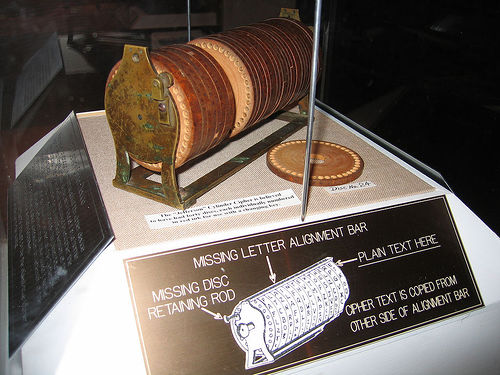
\includegraphics[width=0.4\textwidth]{images/JeffersonDisk.jpg}}
    \hspace{1.5cm}
    \subfloat[Un disque de Jefferson du XVIII\ieme~sicèle au musée
    national de la cryptologie de la NSA]{
      \label{fig:M94}
      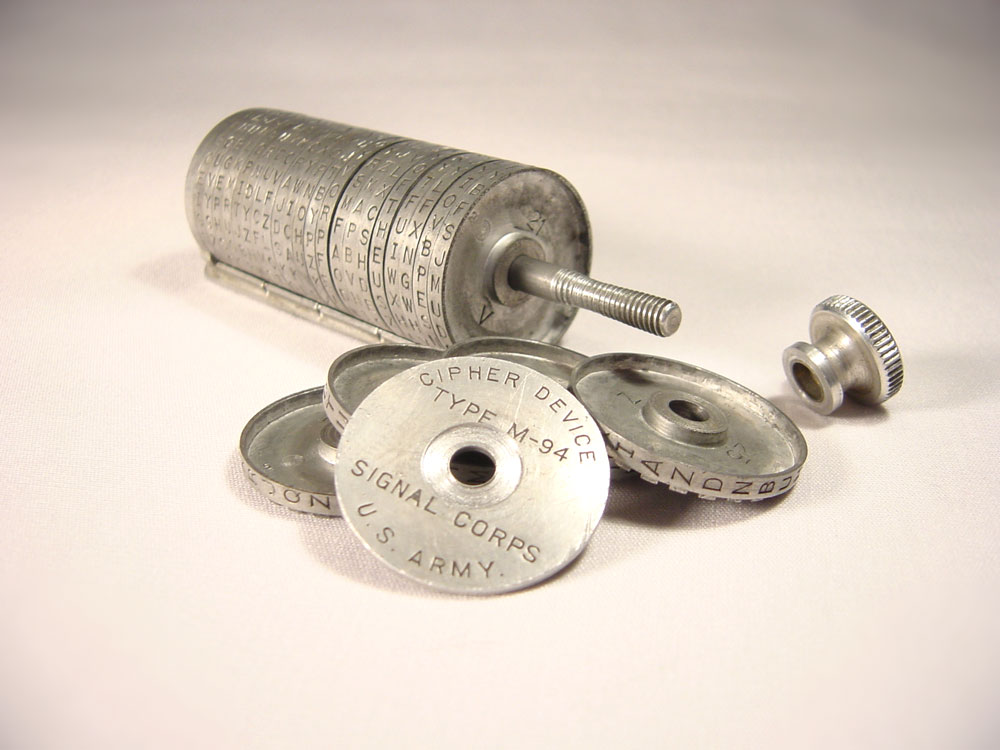
\includegraphics[width=0.4\textwidth]{images/M94.jpg}}
  \end{center}
  \vspace{-10pt}
  \caption{Disques de chiffrement}
  \vspace{-10pt}
  \label{fig:JeffersonDisks}
\end{figure}

Fin XIX\ieme, Charles Wheatstone invente un chiffre
polygrammique que nous verrons en détails plus tard, ce chiffre
portera le nom de la personne l'ayant popularisé : le chiffre
  de Playfair. \\

Ensuite, viennent plusieurs avancées cryptanalytiques avec, comme nous
l'avons vu plus haut, Charles Babbage qui casse le chiffre de
Vigenère, mais ne publie pas sa découverte. Friedrich Kasiski
le casse aussi (sans avoir connaissance des travaux de
Babbage) en 1861, et publie ses travaux. En 1891, Étienne
  Bazeries casse quant à lui le Grand chiffre de Louis XIV. 

En 1883, Auguste Kerckhoffs publie deux articles sur la
cryptographie militaire, où il explique des règles qui peuvent être
considérées comme les règles de base d'un système cryptographique
sûr. Nous verrons ces règles en détail dans le chapitre
\ref{sec:PrincipeKerckhoffs}. \\
\clearpage
\section{La cryptographie pendant la Première Guerre mondiale}
La cryptographie était très présente pendant les guerres, d'où
l'importance des cryptanalystes. Pour cela, chaque état avait recours
à ses cryptanalystes pour décoder les messages ennemis interceptés (ou
même alliés, c'était le cas de l'Angleterre qui écoutait les
communications entrantes et sortantes aux États-Unis).

L'organisme de déchiffrement sûrement le plus important lors de cette guerre
est connu sous le nom de \emph{Room 40} (Bureau 40), le service de
déchiffrement britannique de la \emph{Royal Navy}, qui aurait déchiffré
plus ou moins 15.000 communications allemandes, la plus grosse affaire
connue étant celle du télégramme de Zimmermann.
%\begin{figure}[h]
\begin{wrapfigure}{R}{0.5\textwidth}
  \begin{center}
    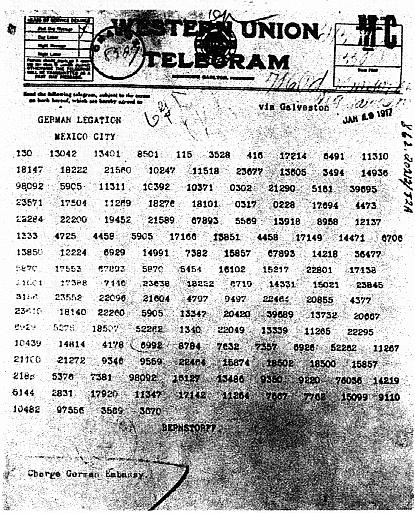
\includegraphics[width=0.48\textwidth]{images/ZimmermanTelegram.jpg}
  \end{center}
  \caption{Photo du télégramme original envoyé par Zimmermann}
  \label{fig:Zimmerman}
  \vspace{-10pt}
%\end{figure}
\end{wrapfigure}


Zimmermann était le ministre allemand des affaires étrangères durant la
guerre. En janvier 1917, alors que les États-Unis sont neutres,
Zimmermann envoie un message codé à l'ambassadeur du Mexique des
États-Unis, qui devrait être retransmis au président Mexicain après
avoir été déchiffré, message qui est intercepté par les services
secrets britanniques, qui charge immédiatement le Bureau 40 du
déchiffrement du message. Un mois plus tard, c'est chose faite ; le
message indiquait que les allemands souhaitaient déclencher une guerre
sous-marine totale, et qu'il serait difficile que les États-Unis
restent neutres. L'empire Allemand propose alors une alliance avec le
Mexique, avec une aide financière pour reconquérir le Texas, le
Nouveau-Mexique et l'Arizona. Il était aussi demandé d'essayer de
convaincre les Japonais d'entrer en guerre contre les États-Unis.
Le message est finalement transmis aux gouvernement américain après
quelques démarches évitant aux anglais de devoir dire aux américains
qu'ils écoutaient leurs communications diplomatiques, et le télégramme
fut publié dans la presse américaine le $1^{er}$ mars. Le 6 avril, les
États-Unis rentrent en guerre contre l'Allemagne, le Congrès ayant
accepté la demande du président Wilson. Bien que le télégramme n'est
pas la seule cause de l'entrée en guerre des États-Unis, il fit
fortement évoluer l'opinion publique américaine dans un sentiment
anti-allemand.

Le Bureau 40 fusionnera après la guerre avec le MI1 (département des
services secrets britannique chargé du décryptage) pour former le
\emph{Government Code and Cypher School}, qui sera encore utile
pendant la Seconde Guerre mondiale, sous le nom de \emph{Government
  Communications Headquarters} \\

En 1917, Gilbert Vernam invente le \emph{masque jetable}, le
seul procédé cryptographique connu comme étant impossible à casser. Ce
procédé n'est pas directement utilisé car il pose des difficultés de
mise en place (problèmes de génération et de transmission des clés,
qui doivent être uniques) \\%TODO: voir en détail ?

%TODO: Room 40 (codebreakers, p 127 -> 150)
% Room 40 : nom du service de déchiffrement de la Royal Navy
% britannique des codes ennemis
%  déchiffré ± 15000 message
% rôle important : savoir les mouvements de la flotte allemande
% Plus grosse affaire : télégramme Zimmerman
% Fusionne avec le MI1 en 1919, sous le nom de Government Code and
% Cypher School, qui sera utile pendant la seconde WW, sous le nom de
% Government Communications Headquarters
% (MI1 : mis en place pendant la guerre, c'est le département des
% services secrets britanniques chargé du décryptage.)
% Zimmerman
% Janvier 1917, États Unis neutres
% Un message codé envoyé par Arthur Zimmerman, ministre allemand des
% affaires étrangères à destination de l'ambassade du mexique, à
% Washington
%  est intercepté par les services secrets et le room 40 est
% chargé du déchiffrement du message. Un mois après, ils y parviennent.
% Le message destiné à l'ambassadeur du mexique aux états unis
% indiquait que les allemands souhaitaient déclencher une guerre
% sous-marine totale, mais qu'il serait difficile que les états-unis
% restent neutres. L'empire allemand propose donc une alliance avec le
% mexique, qui sera aidé financièrement pour reconquérir le Texas, le
% Nouveau Mexique et l'Arizona. Le président devait aussi essayer de
% convaincre les Japonais d'entrer en guerre contre les USA.
% Le message devait être retransmit au
% président amériquain.
% Une fois ce message décodé, tout de suite envoyé aux états unis. La
% presse répand la nouvelle est les US rentrent en guerre le 6 avril
% 1917
% Ils remarquèrent que le message utilisait une technique de
% chiffrement utilisée uniquement pour les communication diplomatique
% importantes, ils se lancèrent donc d'urgence dans le déchiffrement
% du message. Le décodage fut loin d'être simple, mais le mesage
% présentait des similitudes avec d'autres messages interceptés
% auparavant. En combinant tout cela ensembles, ils réussirent petit à
% petit à décoder le message.
%TODO:image

% Chiffre de Playfair réutilisé par les anglais
% Une version complexe du chiffre de Vigenère par les russes, cassée
% en trois jours par Hermann Pokorny
Durant la Première Guerre mondiale, de nombreux systèmes de
chiffrements utilisés étaient pour la plupart d'anciens systèmes de
chiffrements, soit réutilisés tels quels, comme le chiffre de Playfair
repris par les anglais, ou bien modifiés, comme ce fut le cas
avec les russes qui utilisaient une version complexe du chiffre de
Vigenère.\\

Il en est de même pour le système de chiffrement ADFGX, inventé en
mars 1918 par le colonel allemand Fritz % TODO: lieutenant ? (kahn)
Nebel, qui combine une version modifiée
du carré de Polybe\footref{syst:CarrePolybe} (où les chiffres des
lignes et des colonnes sont remplacés par les lettres ADFGX) suivit d'une
transposition\footref{sec:Transposition} (on change la disposition
des colonnes du carré de Polybe). Les lettres ADFGX furent choisies de
façon à limiter le risque d'erreur de l'opérateur qui les
transmettrait en Morse (Nebel trouvait qu'elles étaient les lettres
les plus simples à retenir quand on apprenait le Morse).

Ce système est déchiffré avec beaucoup de difficultés par le
lieutenant français Georges Painvin en avril de la même année, mais à
partir du mois de juin, les allemands compliquent le système
cryptographique en y introduisant la lettre V (ce système se nomme
alors ADFGVX). Le tableau de $5\times 5$ cases devient alors un tableau
de $6\times 6$ cases, ce qui permet l'introduction des chiffres dans
les message codés, et de rendre la cryptanalyse plus
compliquée.

Néanmoins, Painvin parvint à casser le code en moins de
deux jours. Cette cryptanalyse aurait permit d'arrêter l'offensive
des allemands de printemps 1918 et aurait été une étape décisive pour
la victoire des Alliés durant cette guerre, mais certaines personnes
ne sont pas d'accord avec cela, affirmant que lorsque Painvin proposa
sa solution au code, l'attaque des allemands avait déjà échoué. 
%TODO: image explicative ?/matrice
\section{La cryptographie pendant la Seconde Guerre mondiale}
À partir des années 1920, de nombreux dispositifs mécaniques sont mis
en place afin de faciliter le chiffrement. La plupart de ces
dispositifs se basaient sur des rotors (des disques où sont imprimées
les lettres de l'alphabet). C'est le cas de la machine \emph{Enigma},
destinée initialement aux civils (inventée en 1919 par Arthur
Scherbius et commercialisée en 1923), mais très vite utilisée par
l'armée allemande à partir des années 30. La plupart des
communications allemandes seront chiffrées via la machine Enigma, d'où
l'intérêt pour les alliés de pouvoir déchiffrer leurs messages.

La machine Enigma effectue une substitution qui change à chaque
lettre, son fonctionnement est basé sur un assemblage d'un tableau de
connection (qui ne fait que permuter quelques lettres, afin de rendre
la cryptanalyse plus difficile), de plusieurs rotors qui effectuent
les permutations des lettres, et d'un réflecteur qui renvoie le courant
sur le panneau lumineux, où la lettre chiffrée s'allume. À chaque
lettre tapée, le premier rotor avance d'une position ; lorsque le
premier rotor a fait un tour complet, c'est le second qui tourne, et
ainsi de suite. Grâce à la combinaison de ces dispositifs, on peut
obtenir plus de $10^{17}$ clés possibles pour une machine à 5 rotors.

La Pologne pouvait déjà déchiffrer des messages chiffrés via Enigma en
1933, mais lorsque 5 ans plus tard, les allemands ajoutent deux rotors
sur les machines, les polonais communiquent leurs travaux aux
britanniques, qui réunissent au manoir Bletchley Park des milliers de
personnes, aussi bien des mathématiciens que des linguistes, des
amateurs de mots croisés, des joueurs d'échecs professionnels, ...
Cette équipe comportait notamment Alan Turing, grand mathématicien
britannique à qui on doit le concept d'ordinateur, qui s'inspire du
travail des polonais pour créer les \emph{bombes de Turing}, qui
permettaient de retrouver le réglage de la machine à utiliser pour
déchiffrer le message, via la « force brute » (nous verrons ceci plus
en détail dans le chapitre \ref{chap:Cryptanalyse} sur la
cryptanalyse) \\

\begin{figure}[h]
  \begin{center}
    \subfloat[Une machine Enigma à 4 rotors]{
      \label{fig:Enigma}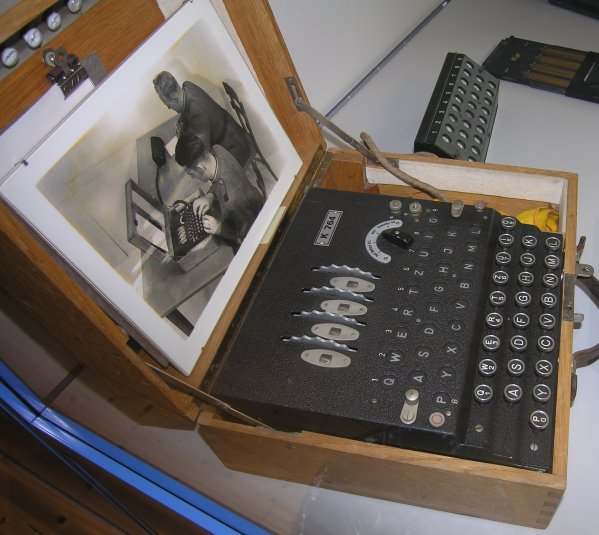
\includegraphics[width=0.4\textwidth]{images/Enigma.jpg}}
    \hspace{1.5cm}
    \subfloat[Les rotors de la Lorenz SZ42]{
      \label{fig:Lorenz}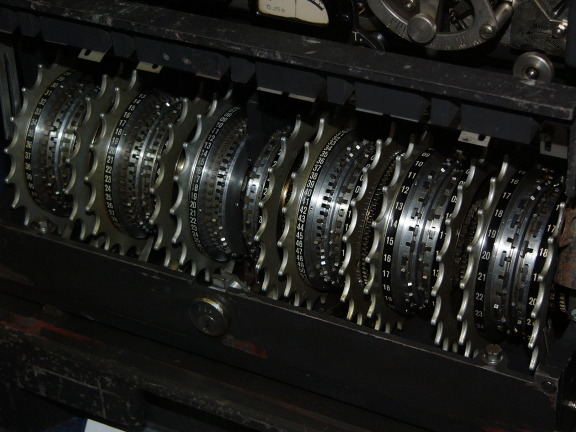
\includegraphics[width=0.4\textwidth]{images/MachineLorenz.jpg}}
  \end{center}
  \vspace{-10pt}
  \caption{Machines à rotors}
  \vspace{-10pt}
\end{figure}


Un autre code utilisé par les allemands (pour les communications entre
les dirigeants) était le Chiffre de Lorenz, via la machine
\emph{Lorenz SZ 40} ou \emph{SZ 42}, surnommée \emph{Tunny} par les alliés. Le
Chiffre de Lorenz est en fait une application du masque jetable de
Vernam, qui nécessite une clé unique par message, et cette clé doit
être une suite de bits aléatoires (on codait les lettres en binaire
via le code Baudot, qui est une table donnant une valeur de 5 bits
pour chaque lettre de l'alphabet et certains caractères
supplémentaires). La machine de Lorenz servait donc à créer des
groupes de 5 bits aléatoires, mais une machine ne peut réellement
produire un résultat aléatoire, on parle alors de nombres
\emph{pseudo-aléatoires}.

Ce chiffre put être cassé grâce à une erreur de la part d'un opérateur
allemand, qui envoya un message de près de 4000 caractères à un autre
opérateur. Le message fut mal reçu par le second opérateur, qui
demanda de le renvoyer à nouveau. Les deux opérateurs ont alors
repositionné leurs machine de Lorenz dans la même position que pour
le message d'avant, alors que le principe du masque jetable est de
n'utiliser chaque clé qu'une seule et unique fois. De plus,
l'opérateur remplaça certains mots par leur abréviation. 

Ces deux erreurs permirent à William T. Tutte, mathématicien anglais
de Bletchley Park, de trouver
facilement la clé utilisée pour ce message, et de comprendre le
fonctionnement de la machine de Lorenz et de découvrir que les clés
produites n'étaient pas réellement aléatoires, ce qu'il explique dans
sa publication \emph{Fish And I}\cite{FISHAndI}
Afin de faciliter le déchiffrement de ces messages, le
premier « ordinateur » électronique, le \emph{Colossus}, fut
construit, et permettait de déchiffrer un message en quelques
heures. \\ 

Pendant que les européens tentaient de casser Enigma et le code de
Lorenz, les américains quant à eux travaillaient sur la machine des
japonais, nommée \emph{97-shiki obun inji-ki} et surnommée \emph{Purple}
par les américains, qui utilisait un système proche des
rotors. William Friedman et son équipe purent reconstruire une machine
Purple à partir des messages chiffrés, en 1940, et arrivèrent casser
les message chiffrés des japonais. Bien qu'ils décodèrent tous les
messages importants pendant la nuit du 6 décembre 1941, ils ne purent
pas éviter l'attaque de Pearl Harbor, aucun message ne disant
clairement d'attaquer à Pearl Harbor. Une alerte fut néanmoins envoyé
à certaines bases américaines avant l'attaque, notamment à celle de
Pearl Harbor, mais ces alertes arrivèrent plusieurs heures après
l'attaque.

\section{La cryptographie moderne}
%TODO: vérifier
Après la guerre, il faudra attendre une trentaine d'années avant de
nouvelles avancées dans le domaine de la cryptologie. 

En 1971, un cryptographe d'IBM, Horst Feistel met au point un
algorithme de chiffrement par bloc, nommé \emph{Lucifer} et qui
possède de nombreuses variantes. Deux ans plus tard, la NSA modifie
\emph{Lucifer} pour sortir le \emph{Data Encryption Standard},
\emph{DES}, en 1977 qui fut encore amélioré par la suite et longuement
utilisé et qui reste utilisé encore aujourd'hui (bien qu'il soit moins
répandu), notemment avec le \emph{Triple DES}, qui consiste
simplemenet à opérer trois DES consécutifs avec deux ou trois clés. %TODO: source

La même année, le chiffrement à clé publique (ou asymétrique) est
présenté pour la première fois dans une publication de W. Diffie et
M. Helmman \cite{NewDirectionsInCryptography} et ce concept est mis en
pratique avec le chiffrement RSA, inventé par Ron Rivest, Adi Shamir
et Leonard Adleman et présenté en 1978 dans une publication 
\cite{RSAPaper}. Grâce aux algorithmes à clé publiques, le problème de
distribution des clés est résolu via l'utilisation de deux clés : une
pour chiffrer, rendue publique, et une pour déchiffrer, gardée secrète
par la personne censée déchiffrer le message.

Par la suite, outre de nouveaux systèmes de chiffrements basés sur des
concepts déjà existants (comme l'\emph{International Data Encryption
  Algorithm}, un chiffrement symétrique apparu en 1990 ou le
\emph{Blowfish}, conçu par Bruce Schneier en 1993, et qui est encore
largement utilisé notemment dans
GnuPG\footnote{\url{http://www.gnupg.org}} et
OpenSSH\footnote{\url{http://www.openssh.com/}}), on peut noter
l'implémentation de la première fonction de hachage en 1989 par Ronald
Rivest, le \emph{R} du RSA, qui conçoit le \emph{Message Digest 2},
MD2 , par la suite amélioré en MD4 et MD5. L'algorithme MD5 est encore
utilisé aujourd'hui, mais de moins en moins suite à des problèmes de
fiabilités. Les fonctions de hachage conseillées aujourd'hui sont les
versions récentes du \emph{Secure Hash Algorithm}, conçut par la NSA à
partir de 1993. Les fonctions de hachage sont utilisées pour vérifier
l'intégrité des données, nous verrons ceci en détail dans le chapitre
les concernant. %(chapitre \ref{sec:Hash})\\
\\

En 1990, l'idée de cryptographie quantique fait son apparition suite
aux résultats de Charles Bennet et Gilles Brassard. Elle permet, en se
basant sur les lois de la physique quantique, de distribuer des clés
en toute sécurité, afin de pouvoir utiliser un chiffre de
Vernam. Ainsi, en mettant en place ce type de cryptographie, un
message pourrait devenir complètement indéchiffrable sans la clé, qui
serait impossible à trouver.

En 1991, Philip Zimmermann sort la première version de \emph{Pretty Good
  Privacy}, PGP, un logiciel de chiffrement et de signature destiné au
grand public, qui combine cryptographie symétrique et asymétrique. Il
explique très bien dans son article « Why I Wrote PGP
»\cite{WhyIWrotePGP} les raisons pour lesquelles il faut utiliser PGP,
en expliquant la volonté du gouvernement américain d'interdire toute
forme de cryptographie sauf une, afin de pouvoir surveiller les
communications du pays entier. Il en conclut qu'il faut utiliser au
maximum la cryptographie tant que c'est légal, car il est difficile de
criminaliser quelque chose de populaire, et que si la cryptographie
est mise « hors-la-loi », seuls les hors-la-loi l'utiliseront, ce qui
ne réglera pas les problèmes. Sa gratuité ayant fait son succès, ce
logiciel est encore largement
utilisé de nos jours, notemment via son implémentation libre, GnuPG. \\

Dans leur publication de 1977\cite{NewDirectionsInCryptography},
Diffie et Hellman remarquent que dans l'histoire, la plupart des
innovations cryptographiques venaient d'amateurs (les machines à
rotors, le disque de Jefferson, \dots) tandis que les professionnels
amélioraient les techniques de cryptanalyse.

Le futur de la cryptographie se tournera donc sûrement vers la
cryptographie quantique ainsi que l'allongement des clés utilisés par
les algorithmes symétriques et asymétriques.
% avec des logiciels
% combinant diverses méthodes de chiffrement (comme le fait PGP)

% La plupart des concepts et méthodes citées ou expliquées brièvement
% dans ce chapitre seront expliqués plus en détails dans les chapitres
% suivants.

% \begin{figure}[h]
%   \begin{center}
%     
\includegraphics[scale=0.2]{images/Puffy.png}
%     \hspace{1cm}
%     \includegraphics[scale=0.3]{images/BruceSchneier.jpg}
%     \hspace{1cm}
%     \includegraphics[scale=1.2]{images/PhilipZimmermann.jpg}
%   \end{center}
%   \caption{De droite à gauche : le poisson lune, emblème de
%     l'algorithme de chiffrement \emph{blowfish}, du logiciel de
%     communications sécurisées \emph{OpenSSH}, et du système
%     d'exploitation mettant l'accent sur la sécurité, \emph{OpenBSD} ;
%     Bruce Schneier, figure importante de la cryptologie actuelle,
%     inventeur de \emph{blowfish} ; Philip Zimmermann, créateur du
%     logiciel PGP}
%   \label{fig:ChiffrementSymetrique}
% \end{figure}
